\chapter{State of the Art}
\label{chap:StateOfTheArt}
\pagestyle{plain}
\vspace{0.5cm}

\noindent This chapter introduces the readers to a complete review of the problem and all the different resolution possibilities.

\section{Physiological signals}
In this section will be defined a general overview on physiological signals that can be used in order to achieve a solution to the Music Emotion Recognition problem.
\\ \indent
Emotions, which affect both human physiological and psychological status, play a very important role in human life. Positive emotions help improve human health and work efficiency, while negative emotions may cause health problems. Long term accumulations of negative emotions are predisposing factors for depression, which might lead to suicide in the worst cases.
\\
The emotion often refers ti a mental state that arises spontaneously rather than through conscious effert and it is accompanied by physical and physiological changes, relevant to the human organs and tissues such as brain, heart, skin, blood flow, muscle, facial expressions, voice, etc. \cite{shu2018review}.
\\ \indent
Emotion recognition has been applied in many areas such as safe driving \cite{de2016enhancing}, health care especially mental health monitoring \cite{guo2013pervasive}, social security \cite{verschuere2006psychopathy}, and so on.
\\
In general, emotion recognition methods could be classified into two major categories:
\begin{itemize}
	\item Using human physical signals such as facial expression \cite{zhang2016facial}, speech \cite{mao2014learning}, gesture, posture, etc. This method has the advantage of easy collecting and is a chapter which has been studied for years. On the other side, the reliability cannot be guaranteed, as it is relatively easy for people to control the physical signals like facial expression or speech to hide real emotions, especially during social communications.
	\item Using internal signals as:
	\begin{itemize}
		\item Electroencephalogram (EEG)
		\item Electrocardiogram (ECG)
		\item Electromyogram (EMG)
		\item Temperature (T)
		\item Blood pressure
		\item Hearth Rate (HR)
		\item Skin Resistance (SR)
		\item Electrodermal Activity (EDA)
		\item Galvanic Skin Response (GSR)
		\item Respiration (RSP)
	\end{itemize}
	These signals are produced by the Nervous System which is divided into:
	\begin{itemize}
		\item Central Nervous System (CNS)
		\item Peripheral Nervous System (PNS): consist of the autonomic and somatic nervous systems (ANS and SNS).
	\end{itemize}
	EEG, ECG, EMG, GSR, RSP and GSR change in a certain way when people face some specific situations. Physiological signals are in response to the CNS and ANS. Due to the fact that CNS and ANS are involuntarily activated, they cannot be controlled.
\end{itemize}
In the table \ref{table:biological_signals} is shown a summary of various papers using different biological signals.
\begin{table}[h!]
	\centering
	\begin{tabular}{|l|l|}
		\hline
		Biological signal & Paper\\ [0.5ex] 
		\hline \hline ECG & \cite{dissanayake2019ensemble}, \cite{hsu2017automatic},  \cite{naji2014classification}, \cite{naji2015emotion}, \cite{cai2009research}  \\ 
		\hline ECG, EMG, RSP & \cite{kim2008emotion} \\
		\hline ECG, GSR & \cite{goshvarpour2017accurate} \\ 
		\hline HR, SR & \cite{yoo2005neural} \\
		\hline EEG & \cite{sourina2012real} \\
		\hline HR & \cite{nardelli2015recognizing} \\
		\hline
	\end{tabular}
	\caption{Papers with correspondent biological signal used}
	\label{table:biological_signals}
\end{table}
\\
The position of different biosensors is shown in figure \ref{fig:biosensors_position}.
\begin{figure}[h]
    \centering
    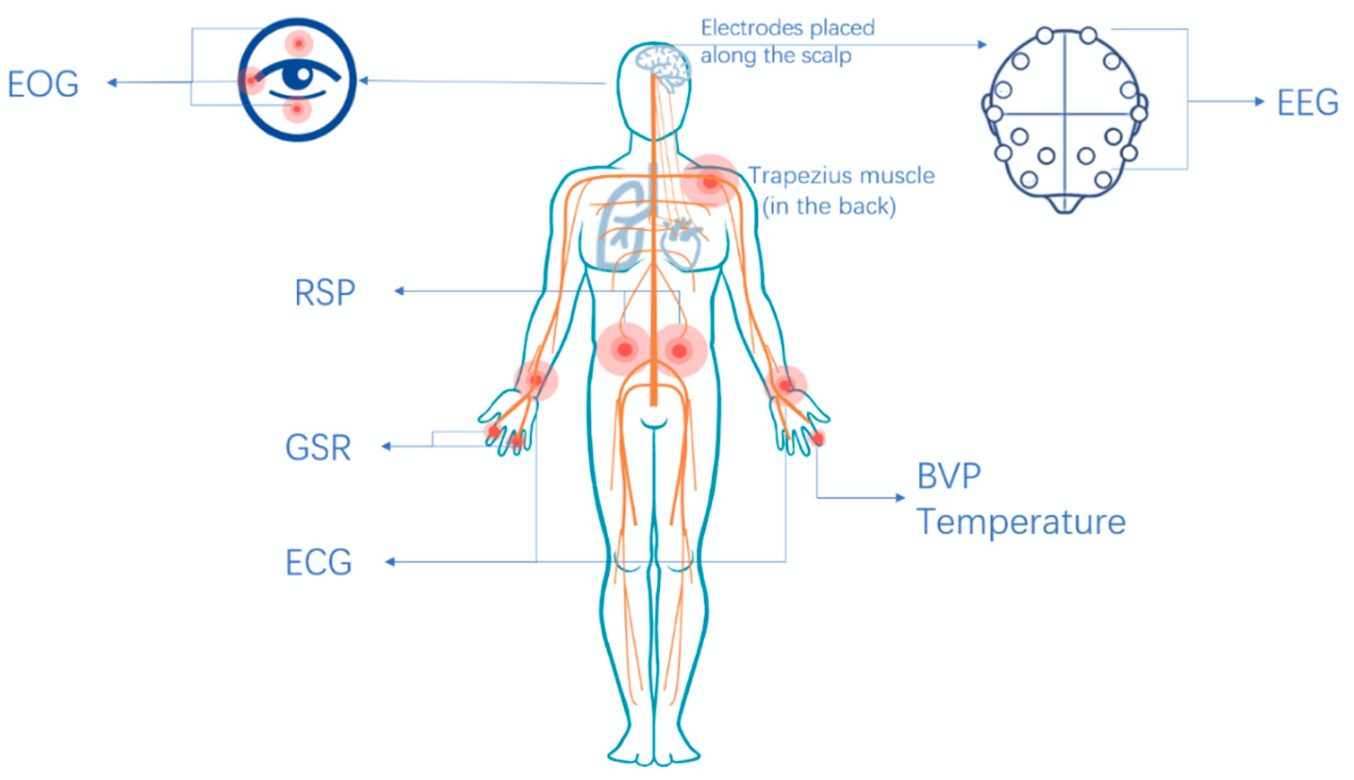
\includegraphics[scale=0.5]{biosensors_position.png} 
	\caption{Position of the bio-sensors}
    \label{fig:biosensors_position}
\end{figure}
Also, in table is presented the relationship between emotions and physiological features, thanks to \cite{shu2018review}.
\begin{table}[h!]
	\centering
	\begin{tabular}{|l|l|l|l|l|l|l|l|}
		\hline
		Signal & Anger & Anxiety & Embarrassment & Fear & Amusement & Happiness & Joy\\ [0.5ex] 
		\hline \hline Cardiovascular &&&&&&& \\ 
		\hline  \\
		
		\hline
	\end{tabular}
	\caption{Papers with correspondent biological signal used}
	\label{table:biological_signals}
\end{table}





